\chapter{Introduction}

Phylogenetics\index{phylogenetics} is the science of studying the evolutionary
relationships (phylogenies\index{phylogenetics!phylogeny}) of a group of organisms~\cite{baldauf03} or genes. One of the fundamental
hypotheses of phylogenetics is that all organisms on Earth had a common ancestor and
can be represented as trees. This hypothesis can be dated back to the era of Darwin
and \lhcomm{is} supported by various studies on the similarity of molecular mechanisms of
organisms~\cite{durbin98}. Successfully reconstructing the tree of life has long been
the dream, and also the aim, of evolutionists.

Traditionally, phylogenetic trees are reconstructed by examining and comparing
morphological characters (both from living and fossilized organisms), which
was and still is a time-consuming and specialized endeavor~\cite{cotton03}.
Since the publication of Zuckerkandl and Pauling's original paper~\cite{zuckerkandl65} that
showed molecular sequences could also serve as characters, molecular phylogenetics
found its own position and has become
a distinct and fruitful direction of phylogenetics in recent years with
rapidly increasing sequence data. It not only
produces \lhcomm{an} overwhelming amount of information to biologists, but also
inspires the development of computer science and statistics.

\section{Background}

Whereas reconstructing the tree of life is one of the central topics of phylogenetics,
reconstructing the phylogeny of each gene family shows the strength of phylogenetic methods
to most of molecular biologists. Phylogenies of gene families not only present
the history of gene evolution, but also hold the key to gene annotations
across species. The functional annotations or experimental results of genes in one
species can be transferred to another when the history of related gene families is
clear. This integrates the efforts of gene annotation in different species and is vital
to annotations, especially to the annotations of a newly sequenced species.
Of the same importance, reconstructing of gene phylogenies is the premise of discovering
the priciples of gene evolution, which further provides clues to interpret gene functions.
For example, the difference of selective pressures on genes implies functional shifts between
them. Meaningful mutations, pseudogenes and interaction networks may also be inferred
with the help of gene phylogenies~\cite{ng03,coin04}. In addition, reconstructing phylogenies of gene families paves
the way for other related evolutionary studies, such as intron evolution and genome-wide
duplications.

Given the importance of gene phylogenies, many databases have been developed to
present the history of each gene family, including KOG~\cite{tatusov03}, PANTHER~\cite{mi05}, SYSTERS~\cite{meinel05}
PhIGs~\cite{dehal05}, Ensembl-compara~\cite{hubbard05}, OrthoMCL~\cite{li03} and HOGENOM~\cite{dufayard05}.
These efforts greatly boost the studies of gene evolution, but they are all faced with
a common problem: how can a reliable phylogenetic tree be reconstructed?
And this problem is, unfortunately, always one of the hardest topics in the area of bioinformatics~\cite{delsuc05}.
Sequences of poor data quality (such as incorrect gene annotation or few informative sites)
and unrealistic underlying evolutionary model (such as assuming that different lineages
have evolved at the same rate) may greatly affect the accuracy of tree building.
No automatic algorithm can reconstruct an accurate tree all the time. To make a phylogenetic database
practically useful, this problem has to be solved.

\section{Overview of the Thesis}

TreeFam is a (gene) tree family database. Phylogenetic trees are the central elements.
In developing TreeFam, the tree building difficulties are solved in two directions. First,
a new algorithm, tree merge, is developed to improve the quality of automatic trees, and second,
mannual curation is applied to further get higher accuracy with the help of the constrained neighbour-joining
algorithm. This thesis presents the details to these algorithms and also covers 
most of topics related to the construction of TreeFam, including
basic concepts, pipelines, additional algorithms, and implementations. In attempt to keep this
thesis as an academic one, technical issues are placed in the appendix even though these
issues might \lhcomm{have been} of the same importance as academic aspects when TreeFam database
was set up.

\begin{figure}
\begin{center}
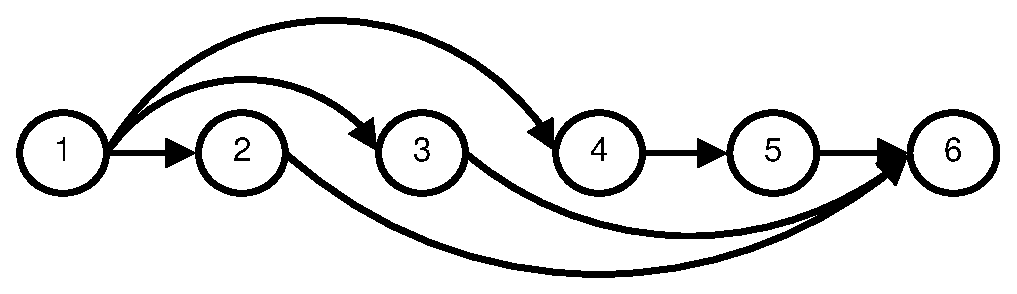
\includegraphics[width=0.7\textwidth]{chapflow}
\caption{Relationships between chapters.}\label{fig:chapflow}
\end{center}
\end{figure}

In the following section of this chapter, \lhcomm{the} biological backgrounds and mathematical
notations will be clarified. Chapter~\ref{chap:treefam} describes the philosophy and structure of \lhcomm{the} TreeFam database.
Chapter~\ref{chap:buildtree} covers various small yet important topics on \lhcomm{the} tree-building process, particularly
two algorithms, constrained neighbour-joinining and leaf reordering algorithm, which
are inspired by \lhcomm{the} TreeFam project. Chapter~\ref{chap:dli} extends the traditional
tree-reconciliation procedure so as to allow for a multifurcated species tree
and presents discussion about tree mapping. Chapter~\ref{chap:merge} describes tree merge algorithms,
which is the chief effort in improving the quality of automatic trees.
And in Chapter~\ref{chap:benchmark}, various tree-building algorithms are evaluated, \lhcomm{using the curated
TreeFam trees as a test set}. The relationships between chapters are showed in Figure~\ref{fig:chapflow}.

Except this introductory chapter, most of the results showed in this thesis have not been published yet.
Although Chapter~\ref{chap:treefam} is based on our paper~\cite{li06}, it still differs much from
the published works. Some important results in the thesis are expected to be published in the following months.

\section{Phylogenetic Terminology}
\emph{Phylogeny}\index{phylogenetics!phylogeny} denotes the evolutionary relationships of a group of organisms or genes.
It can be represented as a tree, called a \emph{phylogenetic tree}\index{tree!phylogenetic tree}.
\emph{Phylogenetics}\index{phylogenetics} is the field of biology that studies phylogenies.
It includes the reconstruction of phylogenies and \lhcomm{the study of the factors that affect
phylogenies, and the biological meaning that phylogenies reveal}.

\begin{figure}[!hb]
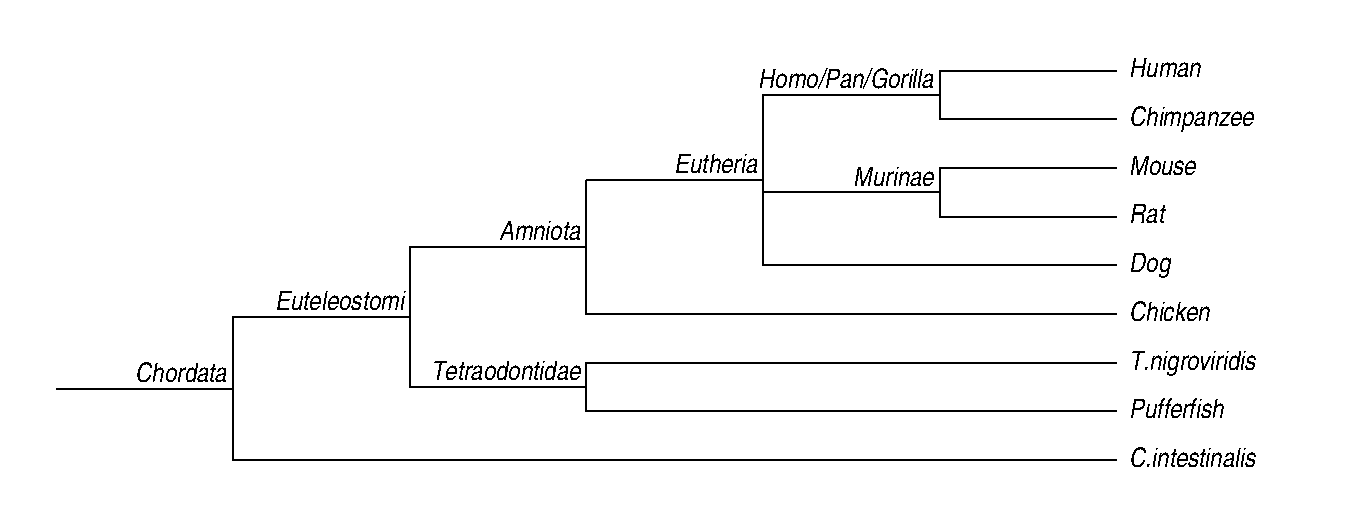
\includegraphics[width=\textwidth]{spec}
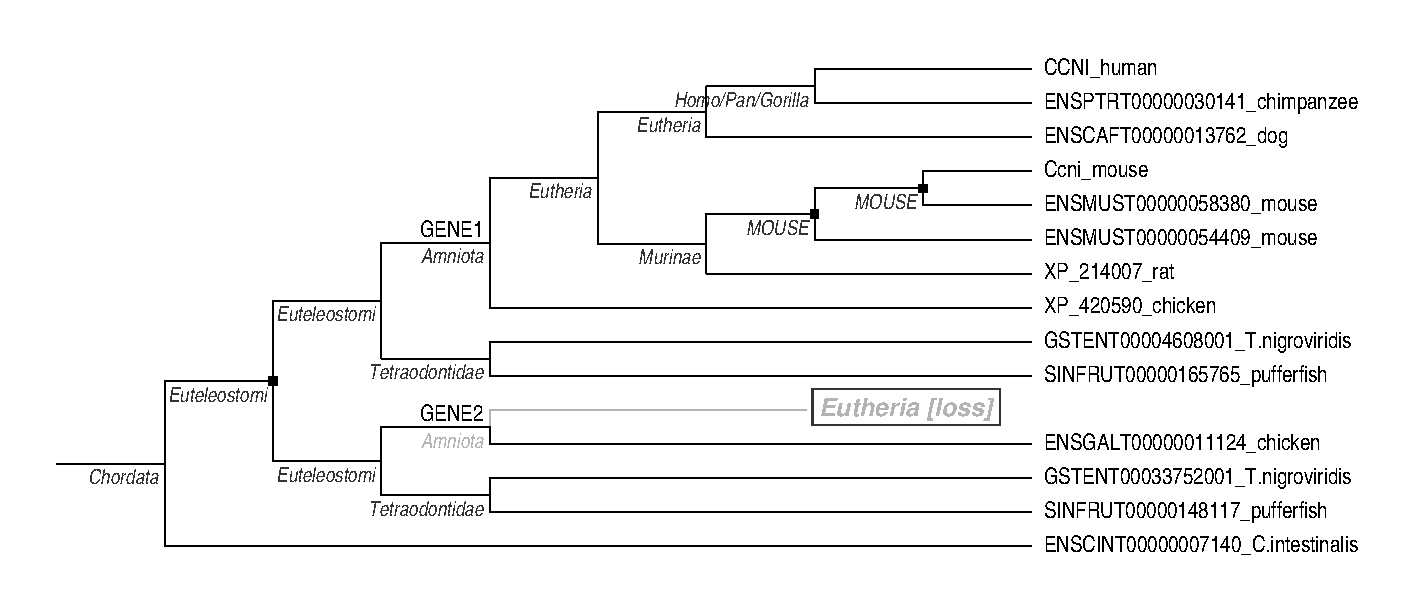
\includegraphics[width=\textwidth]{gtree}
\caption[Examples of a species tree and a gene tree]
	{Example of a species tree and a gene tree. The top figure shows a species tree of {\it Chordata} phylum.
	This tree will be used throughout this thesis.
	The bottom shows the gene tree of {\it Cyclin I} sub- gene family. A slant name beside the internal node
	shows the ancestral species that contained the correponding ancestral gene. In this gene tree,
	the human gene {\sf CCNI\_human} is 1:1 orthologous to {\sf XP\_420590\_chicken} because
	they are descendant from a single gene in {\it Amniota}, the LCA of {\it human} and {\it chicken}. But this human gene is only
	homologous to, but not orthologous to,
	{\sf ENSGALT00000011124\_chicken} because although both genes
	are descendant from a single gene in {\it Euteleostomi}, the human gene is a descendant of {\sf GENE1} in {\it Amniota}
	while {\sf ENSGALT00000011124\_chicken} of {\sf GENE2}. In addition, this gene tree also shows several 1:n orthologs.
	For example, gene {\sf ENSCINT00000007140\_C.intestinalis} is an 1:2 ortholog of {\sf SINFRUT00000165765\_pufferfish}
	and {\sf SINFRUT00000148117\_pufferfish}. The bottom figure will be reexamined in Chapter~\ref{chap:dli}
	where more details will be presented.}\label{fig:spectree}
\end{figure}

In this thesis, two types of trees will be involved: species trees and gene trees.
Strictly speaking, a \emph{species}\index{species}
is ``a group of organisms capable of interbreeding freely with each other but not with members of other
species''~\footnote{\href{http://www.edu.gov.nf.ca/curriculum/teched/resources/glos-biodiversity.html}
{http://www.edu.gov.nf.ca/curriculum/teched/resources/glos-biodiversity.html}}.
A \emph{species tree}\index{tree!species tree} (Figure~\ref{fig:spectree}) describes the evolution relationships between species.
Each of its external nodes (or terminal nodes, or leaf nodes, or leaves)
stands for a present species\index{species!present species} that can be observed nowadays, while each
internal node for an ancestral species\index{species!ancestral species} in history.
An ancestral species is usually named after \lhcomm{the taxon that represents its descendant species}.
For example, when we say species {\it Eutheria}\index{Eutheria@\textit{Eutheria}}, we mean the ancestral species from which
all species in \lhcomm{the taxon {\it Eutheria} are} descendant.
\lhcomm{The} science of naming and classifying organisms is called \emph{taxonomy}\index{taxonomy}, a branch of
phylogenetics.
Taxonomists would prefer to term a (present or ancestral) species as a \emph{taxon}\index{taxonomy!taxon}
({\it pl.} taxa\index{taxonomy!taxa})\footnote{According to taxonomy, all species are classified
at six major levels. In an order from most genernal to most specific, the six levels are
kingdom\index{kingdom}, phylum\index{phylum}, class\index{class}, order\index{order},
family\index{family}, genus\index{genus} and species. For example, {\it human} belongs to
such groups: {\it Animalia} (kingdom), {\it Chordata} (phylum), {\it Mammalia} (class),
{\it Primates} (order), {\it Hominidae} (family), {\it Homo} (genus), and {\it Homo sapiens} (species).}

A \emph{gene}\index{gene} is defined as: ``A DNA segment that contributes to phenotype/function. In
the absence of demonstrated function a gene may be characterized by sequence, transcription or
homology''~\footnote{\href{http://www.gene.ucl.ac.uk/nomenclature/guidelines.html}
{http://www.gene.ucl.ac.uk/nomenclature/guidelines.html}}.
Genes are related in the context of evolution. {\it Homologs}\index{ortholog!homolog} are genes
that are descendant from a single gene~\cite{koonin05}. {\it Orthologs}\index{ortholog} are genes in different
species that originate from a single gene in the last common ancestor of these species~\cite{remm01}; furthermore,
we say $m$ genes in one species and $n$ genes in another form $m:n$ orthologs if
the $m+n$ genes are all descendant from a single gene in the LCA of the two species (Figure~\ref{fig:spectree}).
By definition, orthologs must be homologs, and they are closer homologs;
homologs that are not orthologs are {\it paralogs}\index{ortholog!paralog}.
Homologous genes form a \emph{gene family}\index{gene!gene family} which
is defined a group of gene that are descendant \lhcomm{of} a single ancestral gene. The evolutionary relationships
between genes in a gene family can also be represented as a tree, named \emph{gene tree}\index{tree!gene tree}.
Similarly, each external node of a gene tree stands for a present gene\index{gene!present gene} that
can be observed nowadays, while each internal node for an ancestral gene\index{gene!ancestral gene} that
only existed in history.

Species trees and gene trees are related: species trees can be inferred from gene trees, and
gene trees reflect patterns in species trees. At the same time, gene trees can differ from
species trees due to the existence of duplications\index{duplication}, losses\index{loss}, and
\lhcomm{lateral gene transfer (LGT)}\index{LGT, Lateral Gene Transfer}, which can, in turn, be inferred by reconciling
a gene tree and a species tree. One of the exceptional features of TreeFam, and therefore
of this thesis, is to untangle the relations between species trees and gene trees.
Many meaningful conclusions, such as the functional evolution and differentiation of genes,
can be made when these relations are resolved. Such relations also help to reconstruct reliable gene trees.

% kingdom phylum (subphylum) class (subclass) order (suborder) family genus species
% Animalia Chordata Vertebrata Mammalia Eutheria Primates Catarrhini Hominidae Homo

\section{Terminology \lhcomm{for} Trees}

\subsection{Common terminology \lhcomm{for} trees}
In graph theory, a tree is a connected graph that contains no cycle.
It is comprised of \emph{nodes}\index{node} (vertices\index{vertex}) and \emph{branches}\index{branch}
(edges\index{edge@edge, {\it see also} branch})
which connect nodes. A node can be external\index{node!external node} (terminal\index{node!terminal node})
if it is only attached to one branch,
or internal\index{node!internal node} if two or more branches are joined by the node.
An external node is also termed as a \emph{leaf}\index{leaf}\index{node!leaf node}.

Strictly speaking, every true phylogenetic tree is a \emph{rooted tree}\index{tree!rooted tree} that presents the direction of
evolution. The root\index{node!root node} node is regarded as the earliest ancestor of all the species or genes
in the tree. In a rooted tree, each internal node has its children; except the root, each node has
one parent. The branches close to the root are called higher or deeper
branches\index{branch!deeper branch}\index{branch!higher branch}, while close to
the leaves called lower branches\index{branch!lower branch}.
Given a set of nodes, the lowest ancestral node from which all the given nodes are descendant
is called \emph{LCA} (Last Common Ancestor)\index{LCA, last common ancestor}. A node and
all the nodes descendant from it form a \emph{clade}\index{clade}.

A true phylogenetic tree is also a \emph{binary tree}\index{tree!binary tree} in which each internal node has exactly two children.
A binary tree is also called a \emph{resolved tree}\index{tree!resolved tree} in the sense that every evolutionary event
is presented in the tree. However, if two successive events happened in \lhcomm{a} short time,
they can be hardly discriminated when the tree is reconstructed. In practice, nodes having
three or more children are still allowed. These nodes are called
\emph{polytomies}\index{polytomy@polytomy, \textit{see also} multifurcated node}
or \emph{unresolved nodes}\index{node!unresolved nodes} or
\emph{multifurcated nodes}\index{node!multifurcated node}.
A tree containing polytomies is an \emph{unresolved tree}\index{tree!unresolved tree}
or \emph{multifurcated tree}\index{tree!multifurcated tree}.
The widely used NCBI taxonomy tree~\cite{wheeler05} is a multifurcated tree.

\subsection{Representation of trees}

The most intuitive way to view a tree is to display it as an {\bf image}. However, an image can
neither be directly described in mathematical language nor be easily parsed by a computer program.
Thus it is necessary to introduce abstract languages to shape a tree and to describe
related algorithms as well.

Three types of representations will be used in the thesis: graph representation\index{representation!graph representation},
string representation\index{representation!string representation} and
set representation\index{representation!set representation}. The first two will be explained
here and the third one will appear in Chapter~\ref{chap:merge} where set
representation, being more abstract, helps to clarify the concepts and proof
in a strict manner.

\subsubsection{Graph representation: definitions and notations}

Definitions and notations in this section will be used \lhcomm{throughout} the thesis,
except in Chapter~\ref{chap:merge} where new notations will be introduced
to facilitate specific aims. Only \emph{rooted} \lhcomm{trees} will be discussed here
as any phylogenetic tree is rooted given the assumption that all organisms
on Earth had a common ancestor. In Section~\ref{sec:root-tree}, we
will come to the topic \lhcomm{of} how to find the root of an unrooted tree.

Let $T$ be a \emph{rooted} tree and $V(T)$ be the set of nodes in $T$. \lhcomm{Let $V_E(T)$ and
$V_I(T)$ be} the set of external nodes (or leaves) and internal nodes,
respectively. Given a node $v$, its direct descendants form $\lhchild(v)\subset V(T)$,
$v$'s children set, and $v$ is a child of $\lhparent(v)\in V(T)$, the parent node
of $v$.

For $u,v\in V(T)$, we write $u<v$ or $v>u$ if $u$ is a descendant of $v$. The set
of external nodes that are \lhcomm{descendent} from $v$ is defined as:
\begin{equation}\label{equ:omega}
\omega_T(v)=\{u\in V_E(T):u\leq v\}.
\end{equation}
Similarly, the set of external nodes of set $A\subset V(T)$ form the set:
\begin{equation}
\omega_T(A)=\bigcup_{u\in A}\omega_T(u).
\end{equation}
Sometimes, we might abbreviate $\omega_T(v)$ as $\omega(v)$ if $T$ can be
understood from the context.

Next, we seek to construct a subtree of $T$.
For a node set $A$, we denote by $\lhlca(A)$ the last common ancestor (or LCA)\index{LCA, last common ancestor} of $A$,
which is the lowest node ancestral to all the nodes in $A$. Let $T|_A$ be the subtree\index{subtree}
comprising of only those paths in $T$ that connect $\omega(A)$. Thus, the node set of $T|_A$ is:
\begin{equation}
V(T|_A)=\{v\in V(T):\omega_T(v)\cap\omega_T(A)\neq\emptyset\}
\end{equation}
The root of $T|_A$ is $\lhlca(A)$. We also write $T|_{\{v\}}$ as $T|_v$ for simplicity. Figure~\ref{fig:concept}
shows an example related to these concepts.

\begin{figure}[!hb]
\begin{center}
\setlength{\unitlength}{0.7cm}
\begin{picture}(18,6)
% left
\put(0,2){\line(1,1){4}}
\put(2,2){\line(-1,1){1}}
\put(4,2){\line(0,1){4}}
\put(8,2){\line(-1,1){4}}
\put(6,2){\line(1,1){1}}
\put(-0.2,1.3){1}
\put(1.8,1.3){2}
\put(3.8,1.3){3}
\put(5.8,1.3){4}
\put(7.8,1.3){5}
\put(1.5,2.8){6}
\put(7.5,2.8){7}
\put(4.5,5.8){8}
\put(0,2){\circle{0.1}}
\put(2,2){\circle{0.1}}
\put(4,2){\circle{0.1}}
\put(6,2){\circle{0.1}}
\put(8,2){\circle{0.1}}
\put(1,3){\circle{0.1}}
\put(7,3){\circle{0.1}}
\put(4,6){\circle{0.1}}
% right
\put(14,2){\line(0,1){4}}
\put(18,2){\line(-1,1){4}}
\put(9.8,1.3){1}
\put(11.8,1.3){2}
\put(13.8,1.3){3}
\put(15.8,1.3){4}
\put(17.8,1.3){5}
\put(11.5,2.8){6}
\put(17.5,2.8){7}
\put(14.5,5.8){8}
\put(10,2){\circle*{0.1}}
\put(12,2){\circle*{0.1}}
\put(14,2){\circle{0.1}}
\put(16,2){\circle*{0.1}}
\put(18,2){\circle{0.1}}
\put(11,3){\circle*{0.1}}
\put(17,3){\circle{0.1}}
\put(14,6){\circle{0.1}}
\put(3.8,0){$T$}
\put(13.8,0){$T|_A$}
\end{picture}
\caption[Example tree used to illustrate basic concepts]{Example tree used to illustrate basic concepts.
	In the original tree $T$, $\lhlca(\{4,6\})=8$, and $\omega(8)=\{1,2,3,4,5\}$.
	If $A=\{3,5\}$, the restricted tree $T|_A$ is showed in the right where $V_E(T|_A)=\{3,5\}$
	and $V_I(T|_A)=\{7,8\}$. Note that in $T|_A$, node $7$ only has one child.
	Tree $T$ can be represented as a string in New Hampshire format: {\tt ((1,2)6,3,(4,5)7)8}, or
	{\tt ((5,4)7,(1,2)6,3)8} regardless of the order of leaves. They represent
	the same tree.}\label{fig:concept}
\end{center}
\end{figure}

\subsubsection{String representation: New Hampshire format}\label{sec:nhformat}

New Hampshire (NH) format\index{NH, New Hampshire}, or Newick format\index{format!Newick},
is the standard computer-readable
format to store a \emph{rooted} phylogenetic tree. It makes
use of the correspondence between trees and nested parentheses, and represents a tree
as a string, called an \textbf{NH string}\index{NH, New Hampshire!NH string}.

NH format is clear and intuitive. Figure~\ref{fig:concept} shows how a tree can be represented
as a NH string. The formal grammar of NH format is described as follows:
\begin{quote}
{\tt
\begin{tabular}{lcl}
<tree>	&$\rightarrow$&<cell>\\
<cell>	&$\rightarrow$&<nhcell> | <nhcell>[<comment>]\\
<nhcell>&$\rightarrow$&<node> | <node>:<dist>\\
<node>	&$\rightarrow$&<id> | (<list>) | (<list>)<id>\\
<list>	&$\rightarrow$&<cell> | <list> , <cell>\\
\end{tabular}
}
\end{quote}
where {\tt<comment>}, {\tt<id>} and {\tt<dist>} denote comment, identifier and distance, respectively.
These symbols can be matched by sheer regular expressions and not showed here.
Actually, the tree format used by TreeFam is New Hampshire eXtended (NHX) format\index{NH, New Hampshire!NHX, New Hampshire eXtended}, which
allows for storing additional information in {\tt<comment>} with a specified key-value structure.
NHX format was first suggested by Zmasek {\it et al}~\cite{zmasek012}.

It is important to note that one tree corresponds to many different
NH strings, depending on the order of leaves appearing in the strings. All these
equivalent strings reflect the same topology. In practice, we usually
take as the preferred choice the string in which leaves appear in an order identical
to what is showed in the `image', and so an NH string has a natural 1:1 relation to
the `image' of a tree.

As discussed above, one tree can be displayed in different `image' when plotted on a plane,
or be represented in different NH strings. Although all these images or strings
are equivalent to the same tree, they are quite different in human's eyes. Given two big trees with
hundreds of leaves, it is formidable for a human to discern the difference between them if
the leaves do not appear in similar orders.
To find universal rules to plot a tree is quite necessary, and this is what we will seek
to solve in Section~\ref{sec:reorder}.

\subsection{Comparing two unrooted trees}

Given a set $V$, a \emph{bipartition} of $V$ is a pair of disjoint sets $A|B=B|A$
that satisfy: (i) $A\cap B=\emptyset$ and (ii) $A\cup B=V$.
Let tree $T=(V(T),E(T))$ be an \emph{unrooted} tree whose node (vertex) set is $V(T)$ and
branch (edge) set is $E(T)$. Each branch of $T$ can divides $T$ into two disjoint parts.
If we let the leaf sets of the two disjoint parts be $A$ and $B$, $A|B$ is a bipartition
of $V(T)$. In this way, each branch of $T$ uniquely corresponds to a bipartition of $V(T)$,
and therefore we can construct a set:
\begin{equation}
\tilde{T}=\{A|B:\mbox{there is a branch corresponding to $V(T)$'s bipartition $A|B$.}\}
\end{equation}
Obviously, $|\tilde{T}|=|E(T)|$. As the maximum value of $|E(T)|$ is $2\cdot|V(T)|-3$ when
$T$ is a binary tree, the maximum value of $|\tilde{T}|$ is also $2\cdot|V(T)|-3$.
In the rest of this section, when we say `a branch $A|B$ exists in $T$', we
actually mean that $A|B\in\tilde{T}$, or equivalently, that there is edge corresponding to
the bipartition $A|B$.
Thus the topologies of unrooted trees that have the same leaf set $V$ can be compared.

Let $T_1$ and $T_2$ be two unrooted trees with $V(T_1)=V(T_2)$. The Robinson-Fould distance
measures the topological difference between them, which is defined as:
\begin{equation}
d_T(T_1,T_2)=|(\tilde{T}_1\cup\tilde{T}_2)\setminus(\tilde{T}_1\cap\tilde{T}_2)|
\end{equation}
This distance counts the number of branches that exist in one tree but not in the other.
Note that branches that connect leaves always exist in both $\tilde{T}_1$ and $\tilde{T}_2$, and therefore
the maximum value $d_T$ is $2\cdot(|V(T_1)|-3)$, which can be reached given two totally different
binary trees.

